\documentclass[12pt, letterpaper]{report}
\usepackage{graphicx}
\usepackage{wrapfig}
\usepackage{enumitem}
\usepackage{titlesec}
\usepackage{xcolor}
\usepackage{wrapfig} 
\usepackage{ragged2e}
\usepackage{lmodern}
\usepackage[%
    left=1.25in,%
    right=1.25in,%
    top=0.7in,%
    bottom=1.0in,%
    paperheight=11in,%
    paperwidth=8.5in%
]{geometry}%
\graphicspath{{images/}}
\begin{document}
\title{
\begin{picture}(0,0)
\put(-50,200){
\includegraphics[width=4cm]{he2b}}
\end{picture}
\textbf{Le système de fichiers ext4}}
\author{Costil Iuliana}
\date{Mai 2023}
\maketitle
\tableofcontents
\titleformat{\chapter}[display]
  {\normalfont\LARGE\bfseries\sffamily\centering}{\chaptertitlename\ \thechapter}{0pt}{\LARGE}
\titlespacing*{\chapter}{0pt}{-30pt}{10pt}
\titleformat{\section}
{\normalfont\Large\selectfont\sffamily\raggedright}{\thesection}{1em}{}
\titleformat{\subsection}
{\normalfont\large\selectfont\bfseries\sffamily\raggedright}{\thesubsection}{1em}{}
\chapter{Introduction}
\justifying
Ext4 (quatrième système de fichiers étendu) est un système de fichiers journalisé pour Linux, développé pour succéder à ext3. Ext4 intègre amélioration de l'évolutivité et de la fiabilité pour la prise en charge de systèmes de fichiers volumineux (64 bits) en accord avec l'augmentation des capacités de disque et l'état de l'art exigences de fonctionnalité.
\section{L'évolution des systèmes de fichiers ext}
\begin{enumerate}
  \item ext : le premier système de fichiers ext a été introduit en 1992 dans le cadre du noyau Linux. Il prenait en charge les noms de fichiers jusqu'à 255 caractères et avait une taille de fichier maximale de 2 Go. Il a également introduit des fonctionnalités telles que la prise en charge des liens symboliques et des autorisations de fichiers.
  \item ext2 : En 1993, ext2 a été publié, ajoutant la prise en charge de fichiers de plus grande taille jusqu'à 2 To et améliorant les performances grâce à des fonctionnalités telles que les descripteurs de groupes de blocs, qui ont amélioré les temps d'accès au disque. Il a aussi introduit la journalisation, qui a permis une récupération plus rapide en cas de panne du système ou de panne de courant.
  \item ext3 : en 2001, ext3 a été publié en tant qu'extension d'ext2, ajoutant la prise en charge de la journalisation par défaut. Cela a rendu le système de fichiers plus fiable et réduit le risque de perte de données. Il a de plus introduit la possibilité de convertir un système de fichiers ext2 en ext3 sans perte de données.
  \item 	ext4 : en 2008, ext4 a été publié avec des améliorations significatives en termes de performances et d'évolutivité. Il a ajouté la prise en charge de systèmes de fichiers plus volumineux. Il a également introduit des fonctionnalités telles que l'allocation différée, qui a amélioré les performances d'écriture, et les étendues, qui ont amélioré l'efficacité du système de fichiers en réduisant la fragmentation.
\end{enumerate}

\section{Principales améliorations d'ext4 par rapport à ses prédécesseurs}
\justifying
Ext4 a été introduit pour répondre à certaines des limitations d'ext3 et pour fournir de meilleures performances, fiabilité et évolutivité. Voici quelques-unes des principales améliorations d'ext4 par rapport à ses prédécesseurs :
\newline
\textbf {Augmentation de la taille des fichiers} : Ext4 permet des tailles de fichiers plus importantes que ext3. La taille de fichier maximale dans ext4 est de 16 téraoctets. Dans ext3, la taille de bloc maximale est de 4 Ko. Avec une taille de bloc de 4 Ko, la taille de fichier maximale en ext3 est de 2 To. 
\newline
\textbf {Performances améliorées} : Ext4 utilise une allocation plus efficace de l'espace disque, ce qui peut améliorer les performances lors de la création, de la suppression et du redimensionnement des fichiers. Il utilise également l'allocation différée, ce qui améliore les performances en réduisant la fragmentation du disque.
\newline
\textbf {Meilleure fiabilité} : Ext4 inclut la prise en charge de la somme de contrôle du journal, ce qui permet de détecter et de corriger les erreurs dans le système de fichiers. Il comprend également une fonctionnalité appelée "fast commit", qui réduit le risque de perte de données en cas de panne de courant.
Évolutivité améliorée : Ext4 peut gérer plus de fichiers et de répertoires qu'ext3, et il peut prendre en charge des disques plus grands avec une allocation de blocs plus efficace.
\newline
\textbf {Rétrocompatibilité} : Ext4 est conçu pour être rétrocompatible avec ext3, ce qui signifie qu'il peut être monté en tant que système de fichiers ext3 si nécessaire.
Dans l'ensemble, ext4 représente une amélioration significative par rapport à ext3 en termes de performances, de fiabilité et d'évolutivité. Il s'agit d'un système de fichiers largement utilisé pour Linux et pris en charge par la plupart des distributions Linux modernes.

\chapter{Architecture}
\section{La structure }
\justifying Le système de fichiers Ext4 est constitué d'un bloc de démarrage ainsi que de plusieurs groupes de blocs. Chacun de ces groupes contient plusieurs éléments clés tels que le superbloc, la table de descripteurs de groupe de blocs, le bitmap de blocs, le bitmap d'inodes, la table d'inodes et le bloc de données. Chaque élément remplit une fonction spécifique dans la gestion du système de fichiers et de son contenu. De plus, la redondance est intégrée dans le système pour assurer une fiabilité accrue.

\centering 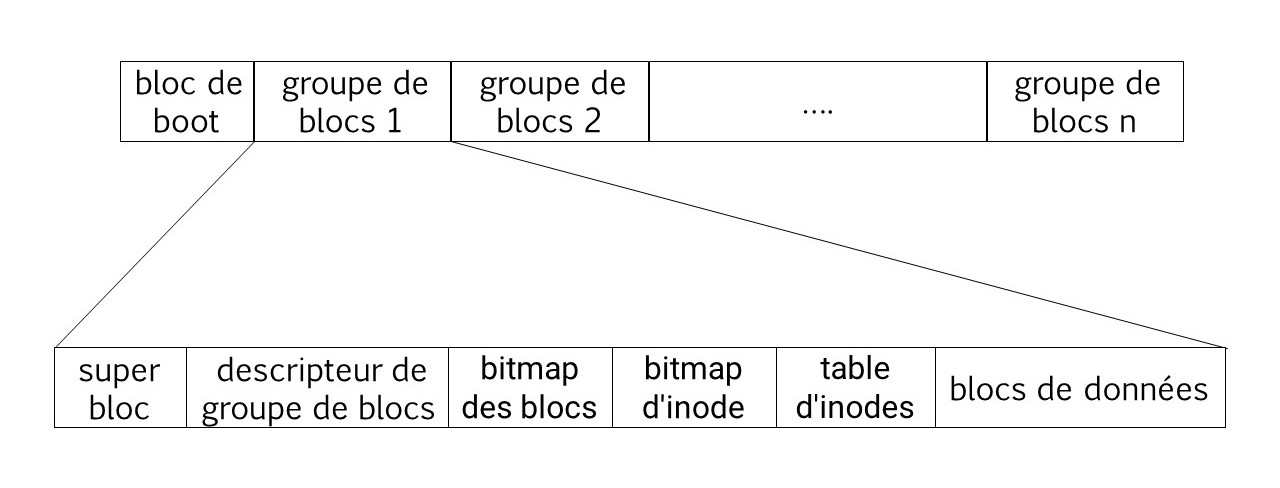
\includegraphics[width=\textwidth]{structure}
\justifying

\underline{Bloc de boot} : le bloc de boot (de démarrage) est le premier secteur du système de fichiers et contient le code du chargeur de démarrage. Il est utilisé pour démarrer le système d'exploitation, il est optionnel. 

\underline{Superbloc} : le superbloc est une structure de données qui contient des informations sur le système de fichiers, telles que sa taille, la taille du bloc, le nombre d'inodes et le nombre de blocs libres. Il est situé à une position fixe dans le système de fichiers et est répliqué plusieurs fois dans tout le système de fichiers pour la redondance.

\underline{Table de descripteur de groupe de blocs} : la table de descripteur de groupe de blocs contient des informations sur chaque groupe de blocs du système de fichiers, telles que le bitmap de bloc, le bitmap d'inode et la table d'inode. Il est situé après le superbloc et est répliqué pour la redondance.

\underline {Bitmap des blocs} : le bitmap de bloc est une carte des blocs de données utilisés et libres dans un groupe de blocs. Il est utilisé pour allouer et désallouer des blocs de données.

\underline{Bitmap d'inode}: le bitmap d'inodes est une carte des inodes utilisés et libres dans un groupe de blocs. Il est utilisé pour allouer et désallouer des inodes.

\underline{Table d'inodes} : la table d'inodes contient les métadonnées de chaque fichier du système de fichiers, telles que le type de fichier, la propriété, les autorisations et les horodatages. Il est utilisé pour localiser les blocs de données qui stockent le contenu réel du fichier.

\underline{Blocs des données} : le bloc de données est l'endroit où le contenu réel du fichier est stocké. Ext4 prend en charge différentes tailles de bloc allant de 1 Ko à 64 Ko, ce qui permet de meilleures performances et une utilisation efficace du stockage.

\section{Groupes de blocs}
\subsection{Superbloc}
Le superbloc est une structure de données qui stocke des informations sur le système de fichiers dans son ensemble, telles que sa taille, son emplacement et son état. Le superbloc est dupliqué au cas où une copie serait endommagée. Il est fixé en place sur le disque et contient les informations suivantes:

\begin{center}
	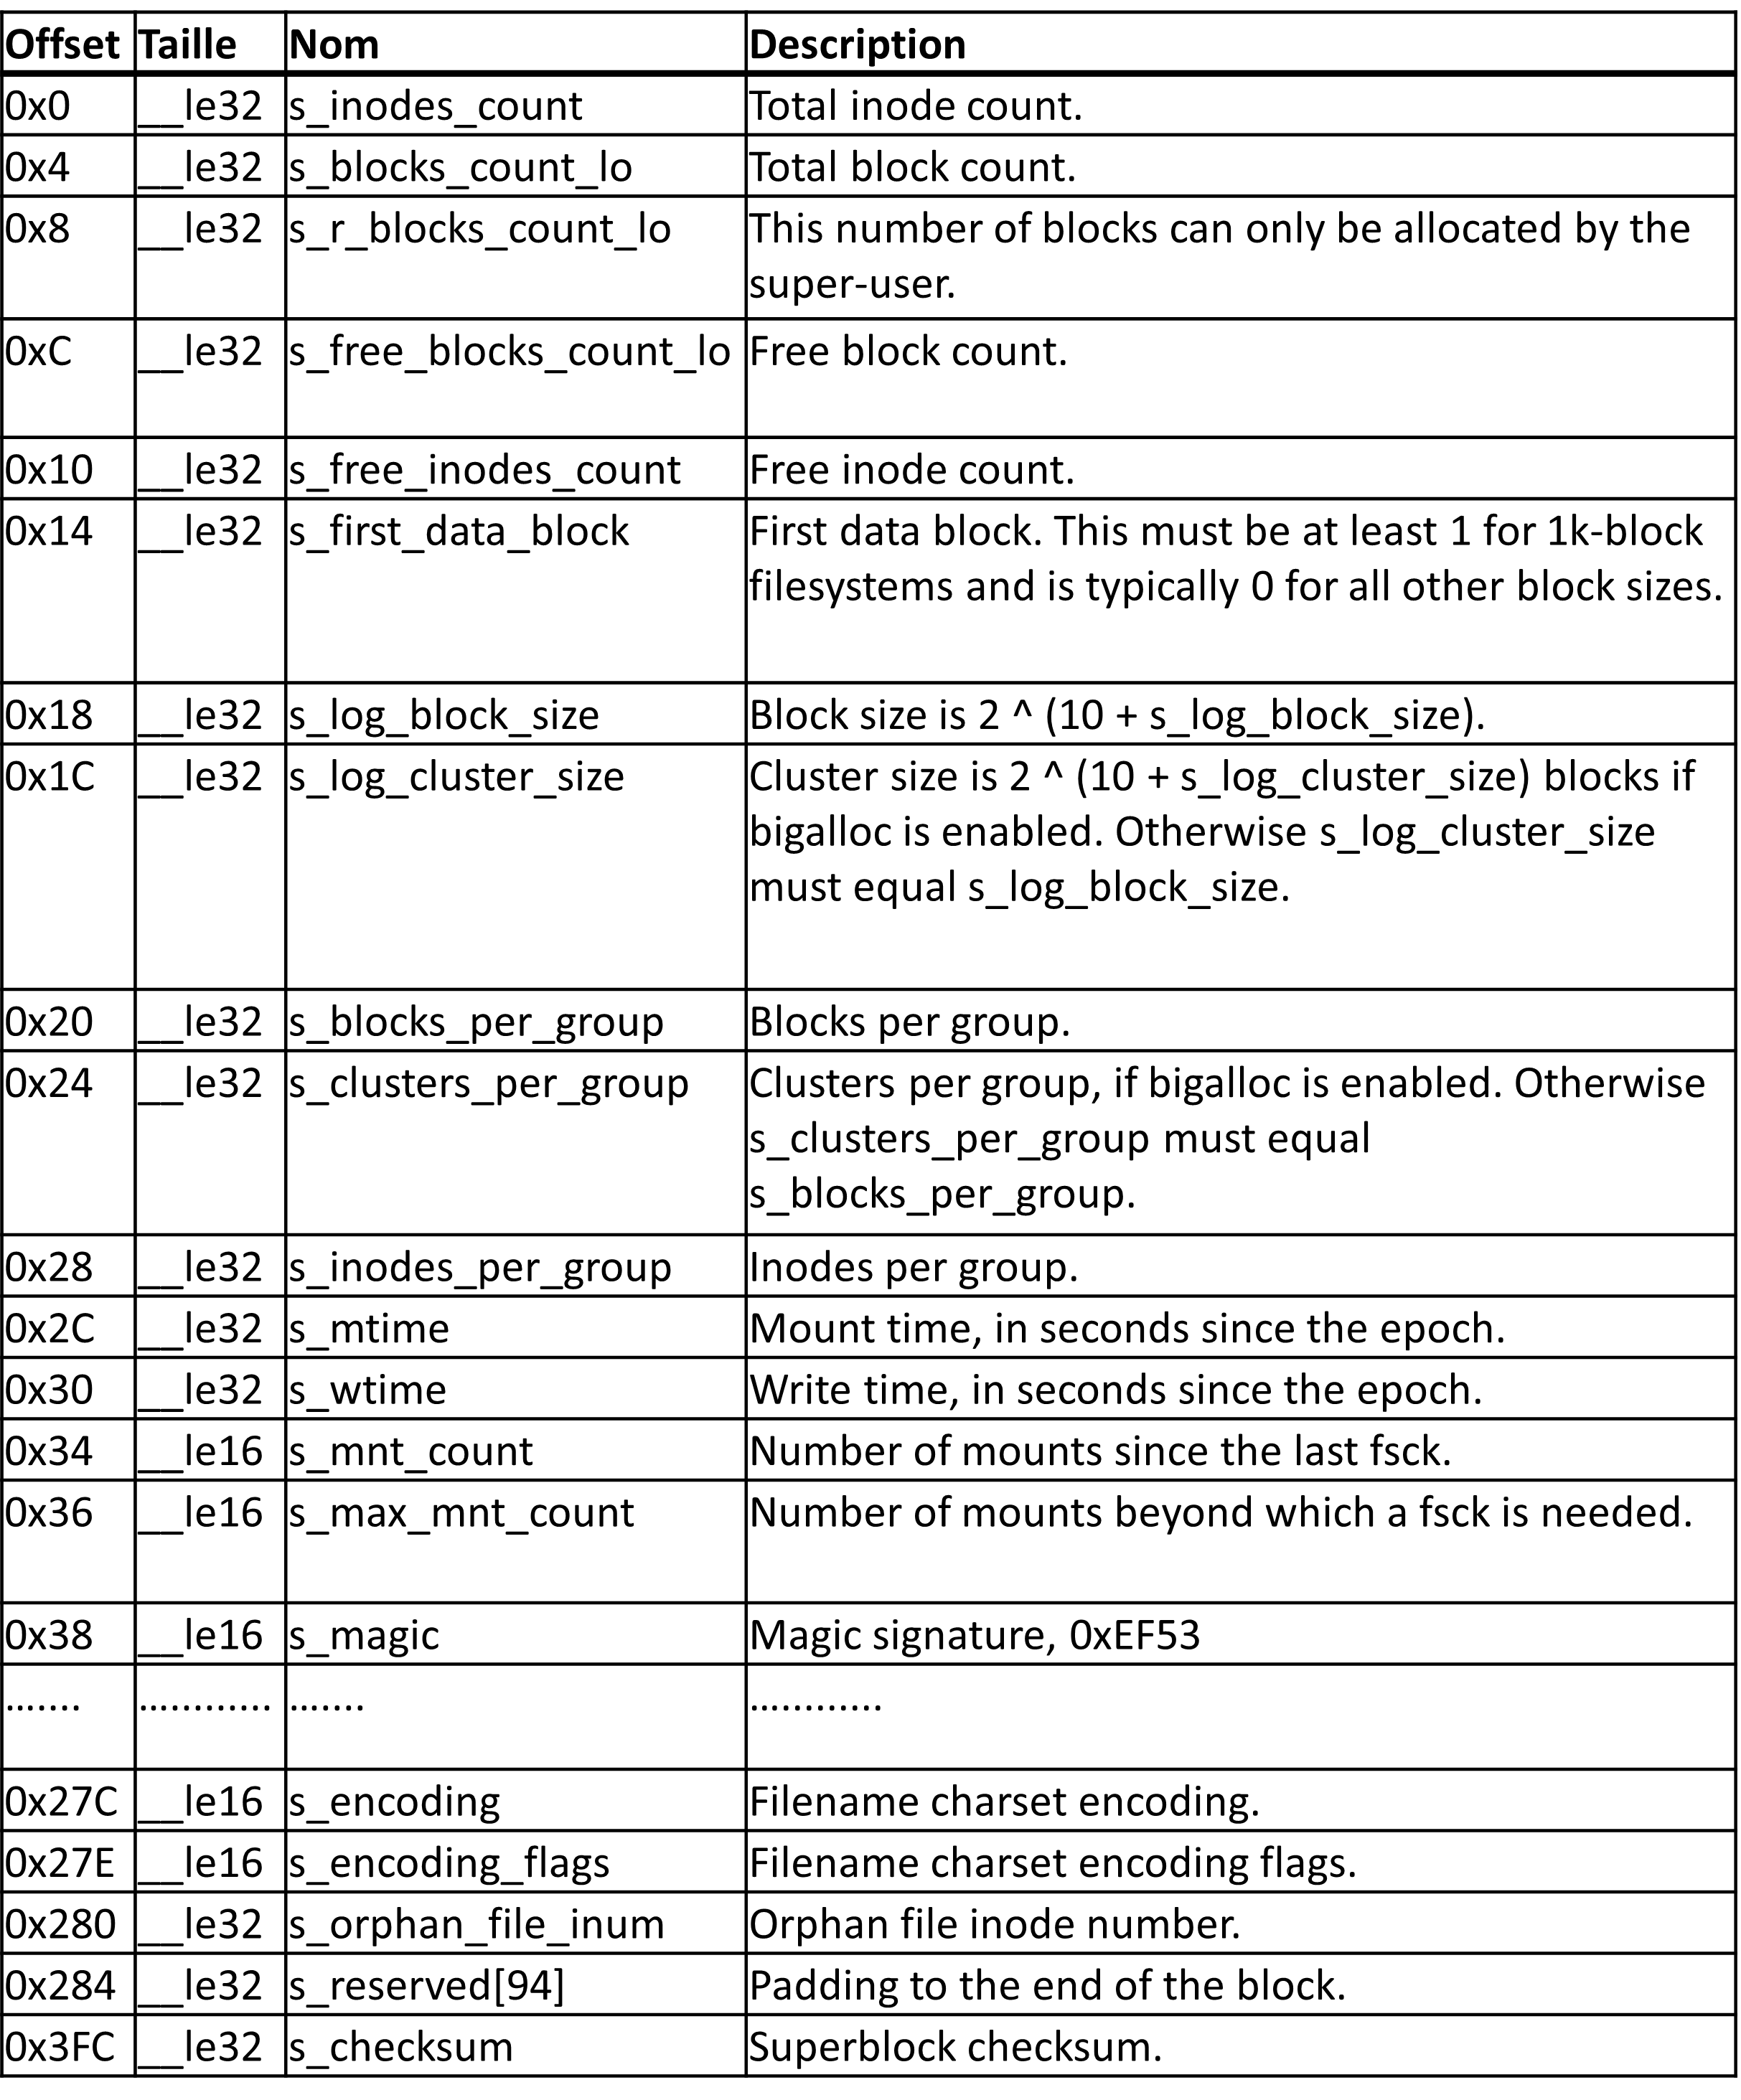
\includegraphics[width=\textwidth]{superbloc}
\end{center}
La taille "le32" signifie "little endian 32 bit integer"

Créons un système de fichiers ext4 pour explorer la structure.
\begin{center}
	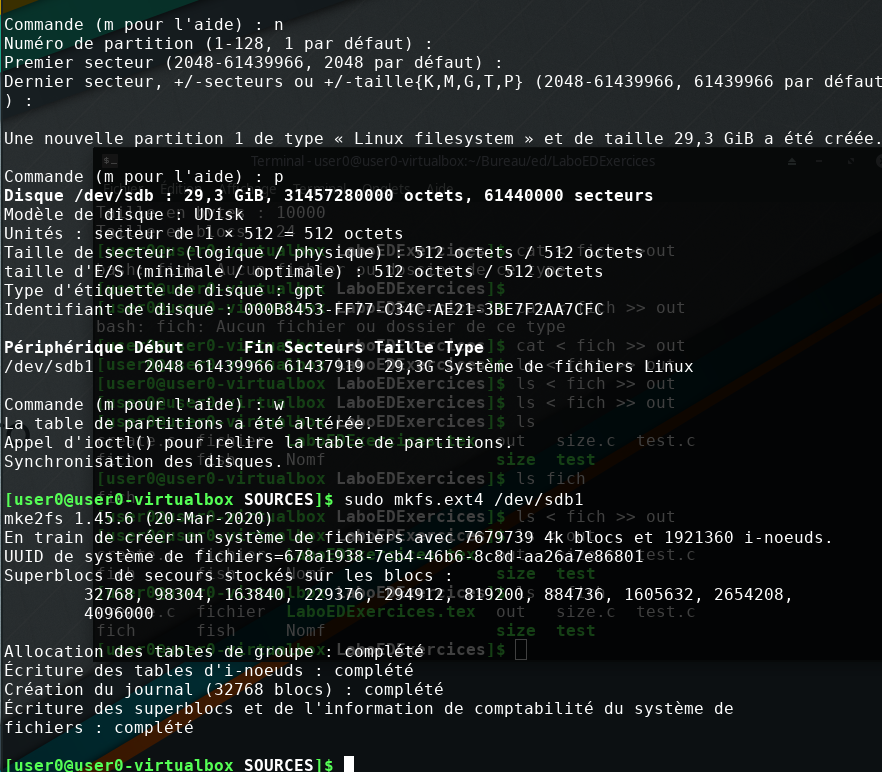
\includegraphics[width=\textwidth]{mount}
\end{center}

Les informations que nous voyons ici sont :\newline
\begin{itemize}
  \item Un système de fichiers est créé composé de 7679739 blocs.
  \item La taille de bloc de 4096B est la valeur automatiquement sélectionnée, nous pouvons également créer avec une autre taille de bloc (-b blocksize). Cette taille de bloc n'est pas la taille de bloc logique (de LBA), c'est la taille de bloc du système de fichiers, et les blocs d'environ 4 M mentionnés ci-dessus sont les blocs du système de fichiers et non les blocs logiques.
  \item Il y a 1921360 inodes.
  \item	L'UUID du système de fichiers est l'UUID de la partition dans GPT.
  \item Il y a quelque chose qui s'appelle Superblock avec 10 sauvegardes. Les groupes de blocs 0, 1 et les puissances de 3, 5 et 7 auront des superblocs de secours (par exemple : 343, 243, 125, 81, etc.)
  \item Il y a des choses appelées tables de groupe, tables d'inodes et journal.
\end{itemize}

Nous pouvons voir le contenu du superbloc avec dumpe2fs et l'option -h n'imprime que le Superblock. LectSuperBloc.c contient un code pour faire ça manuellement.
\begin{center}
	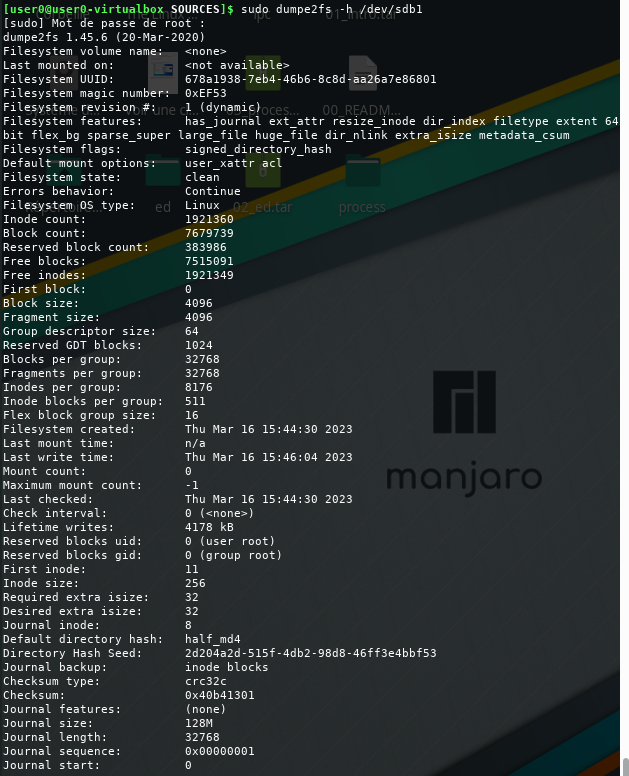
\includegraphics[width=\textwidth]{dumpsuperbloc}
\end{center}


\justifying
Le concept de disposition de stockage le plus basique d'ext4 est Block. ext4 alloue le stockage dans une série de blocs. La taille de bloc dans Superblock est de 4096B = 4KB. Le nombre de blocs dans ce système de fichiers est 7679739. \newline
Le deuxième concept de disposition de stockage de base d'ext4 est le groupe de blocs. Les blocs contigus sont organisés en groupes de blocs, et dans notre système de fichiers, c'est 32768 = 32K.\newline
La taille de bloc est de 4 KB. 8 * 4096 = 32768 blocs alloués par groupe.\newline
Puisque nous avons 7679739 blocs, en divisant cela par 32K : 234,36
Nous avons donc 235 groupes de blocs contenant chacun 32K blocs (sauf le dernier).

\subsection{Descripteur de groupe de blocs}

\begin{center}
	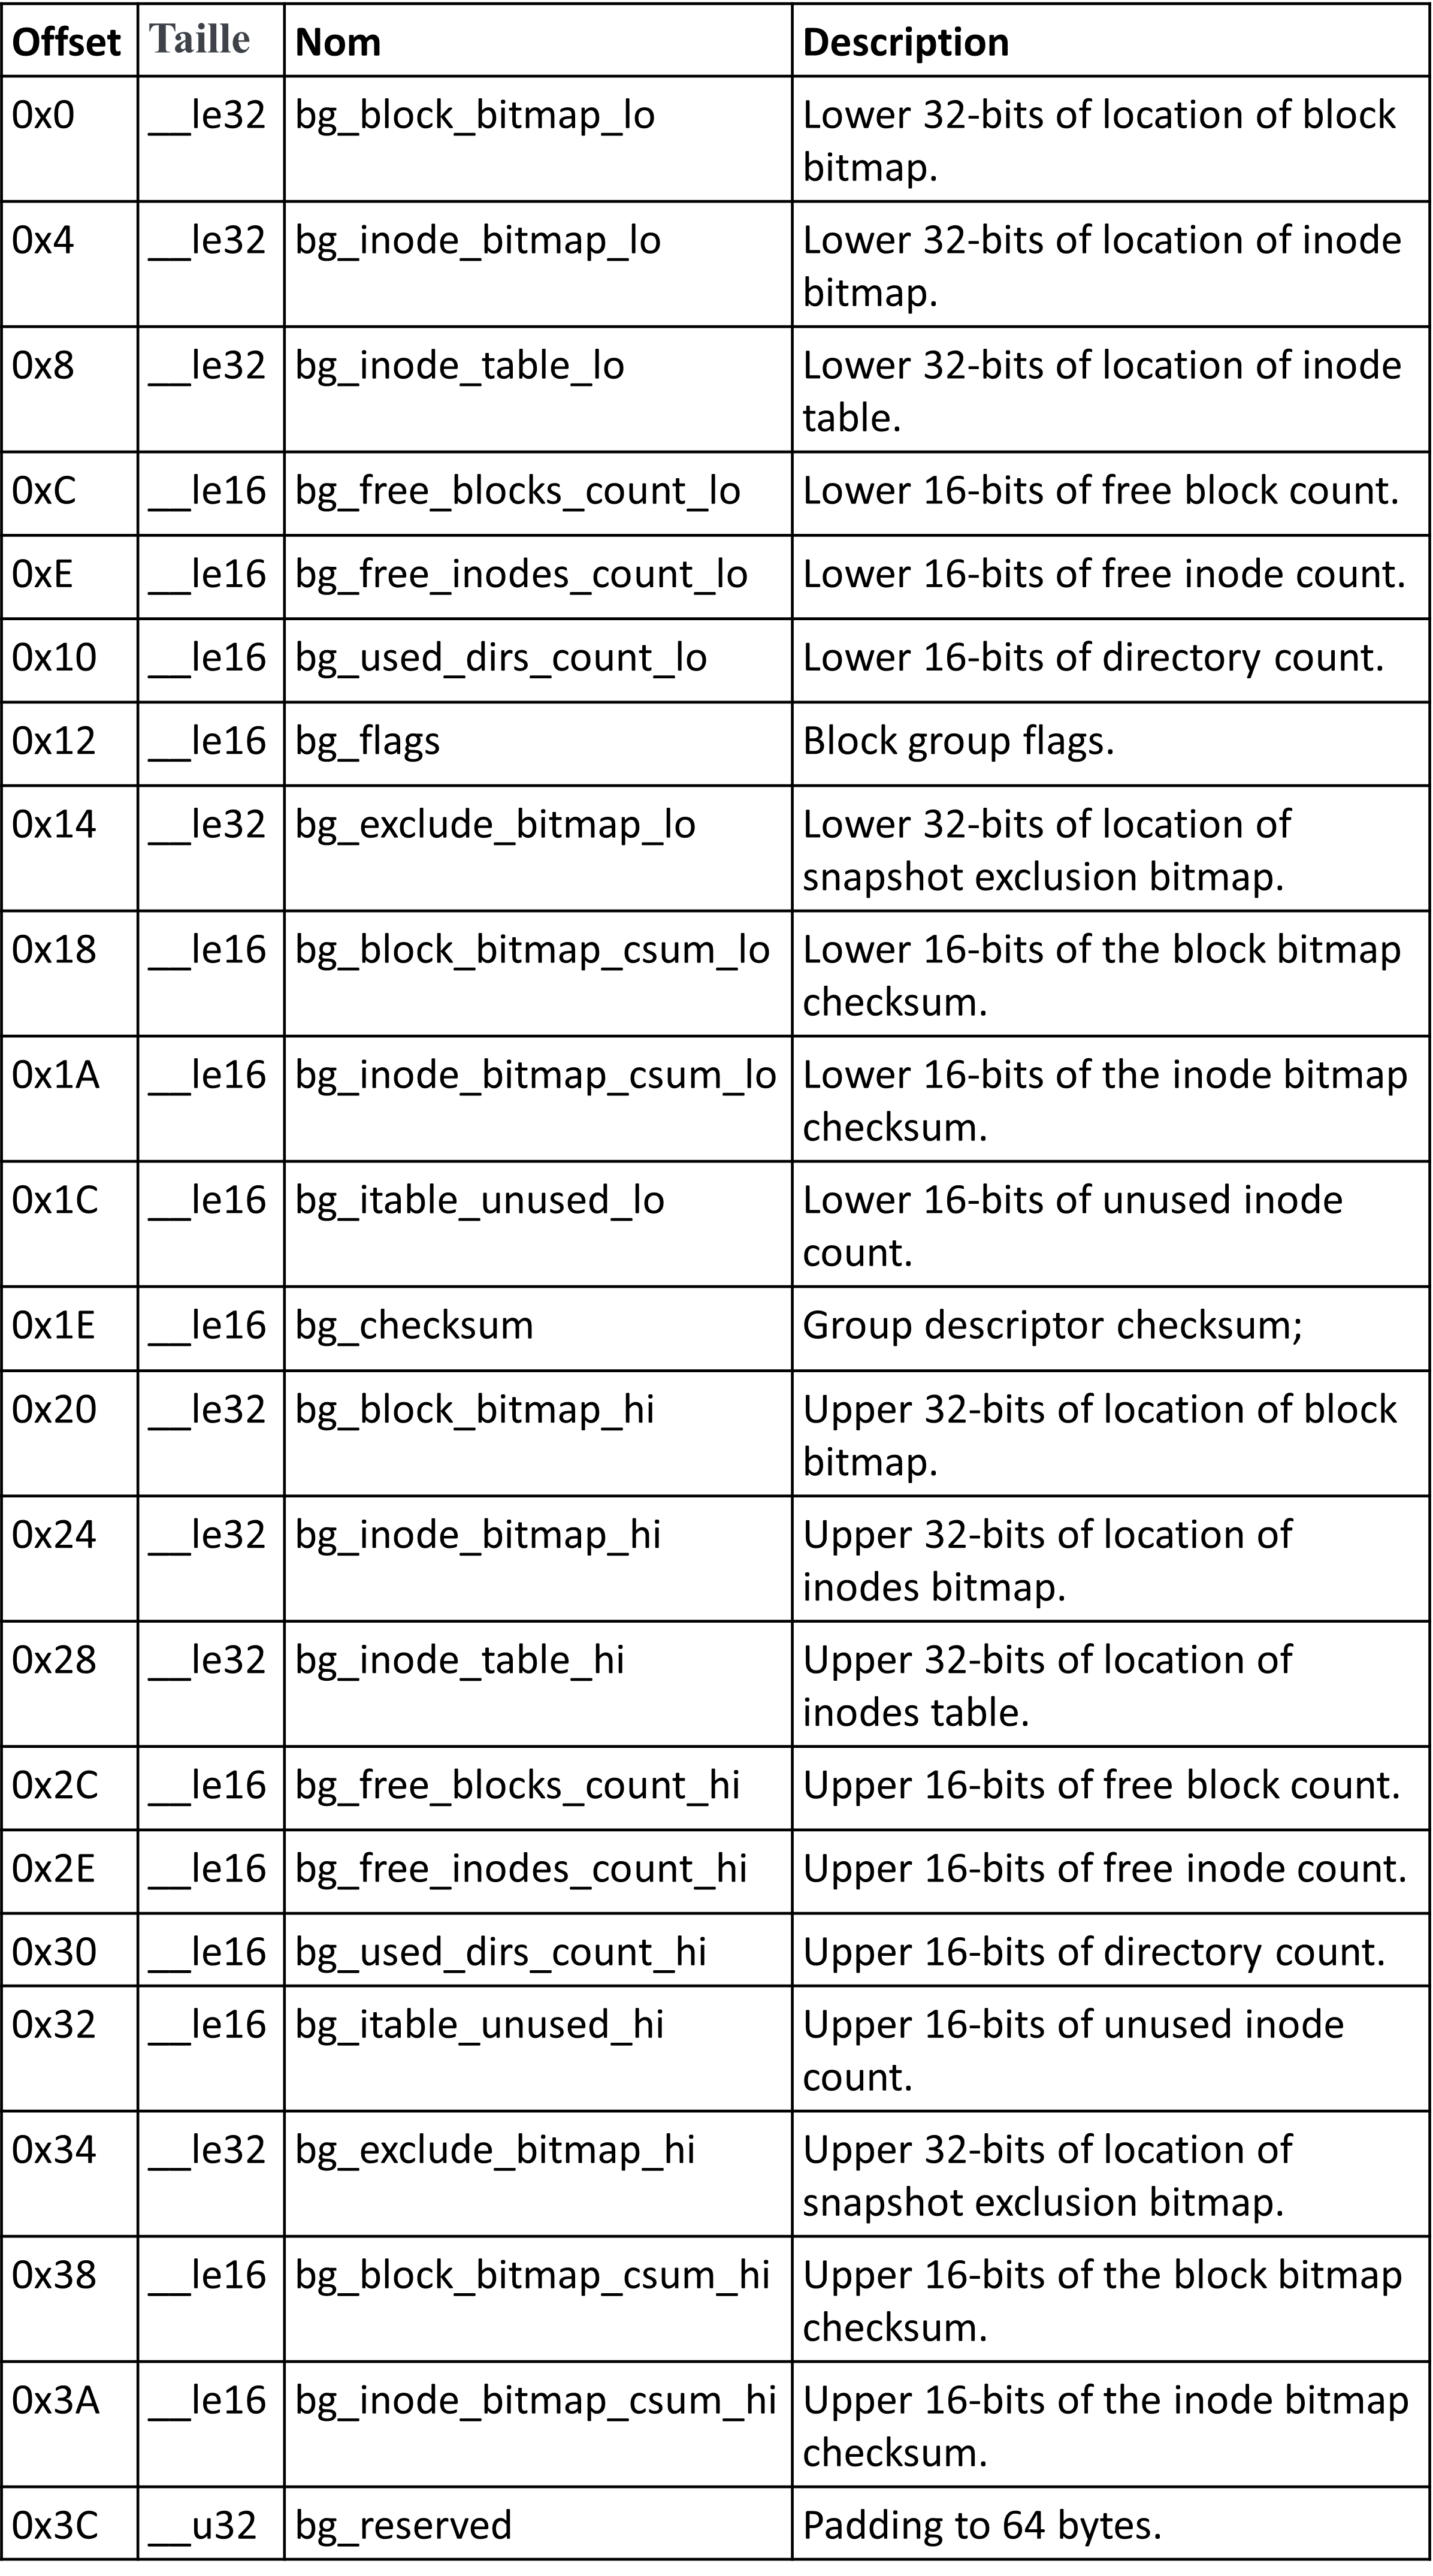
\includegraphics[width=\textwidth]{blockdesc}
\end{center}
Chaque groupe de blocs sur le système de fichiers est associé à l'un de ces descripteurs. Les descripteurs de groupe sont le deuxième élément du groupe de blocs. \newline
Remarquez comment le descripteur de groupe enregistre l'emplacement des deux bitmaps et de la table d'inodes (c'est à dire qu'ils peuvent flotter). Cela signifie qu'au sein d'un groupe de blocs, les seules structures de données avec des emplacements fixes sont le superbloc et la table de descripteurs de groupe. Le mécanisme flex\_bg utilise cette propriété pour regrouper plusieurs groupes de blocs dans un groupe flexible et disposer tous les bitmaps et tables d'inodes des groupes en un seul long terme dans le premier groupe du groupe flexible.

\subsection{Table d’inodes}
Le système de fichiers ext4 prend en charge à la fois l'allocation basée sur l'inode et l'étendue. Dans la méthode d'allocation traditionnelle basée sur l'inode, l'inode contient des pointeurs vers des blocs de données individuels sur le disque. Dans la méthode d'allocation basée sur l'étendue, un seul inode peut représenter plusieurs blocs de données contigus, appelés extents.
La structure d'un inode ext4 avec des extensions ou des pointeurs vers des blocs de données est similaire, avec quelques différences clés.

\begin{center}
	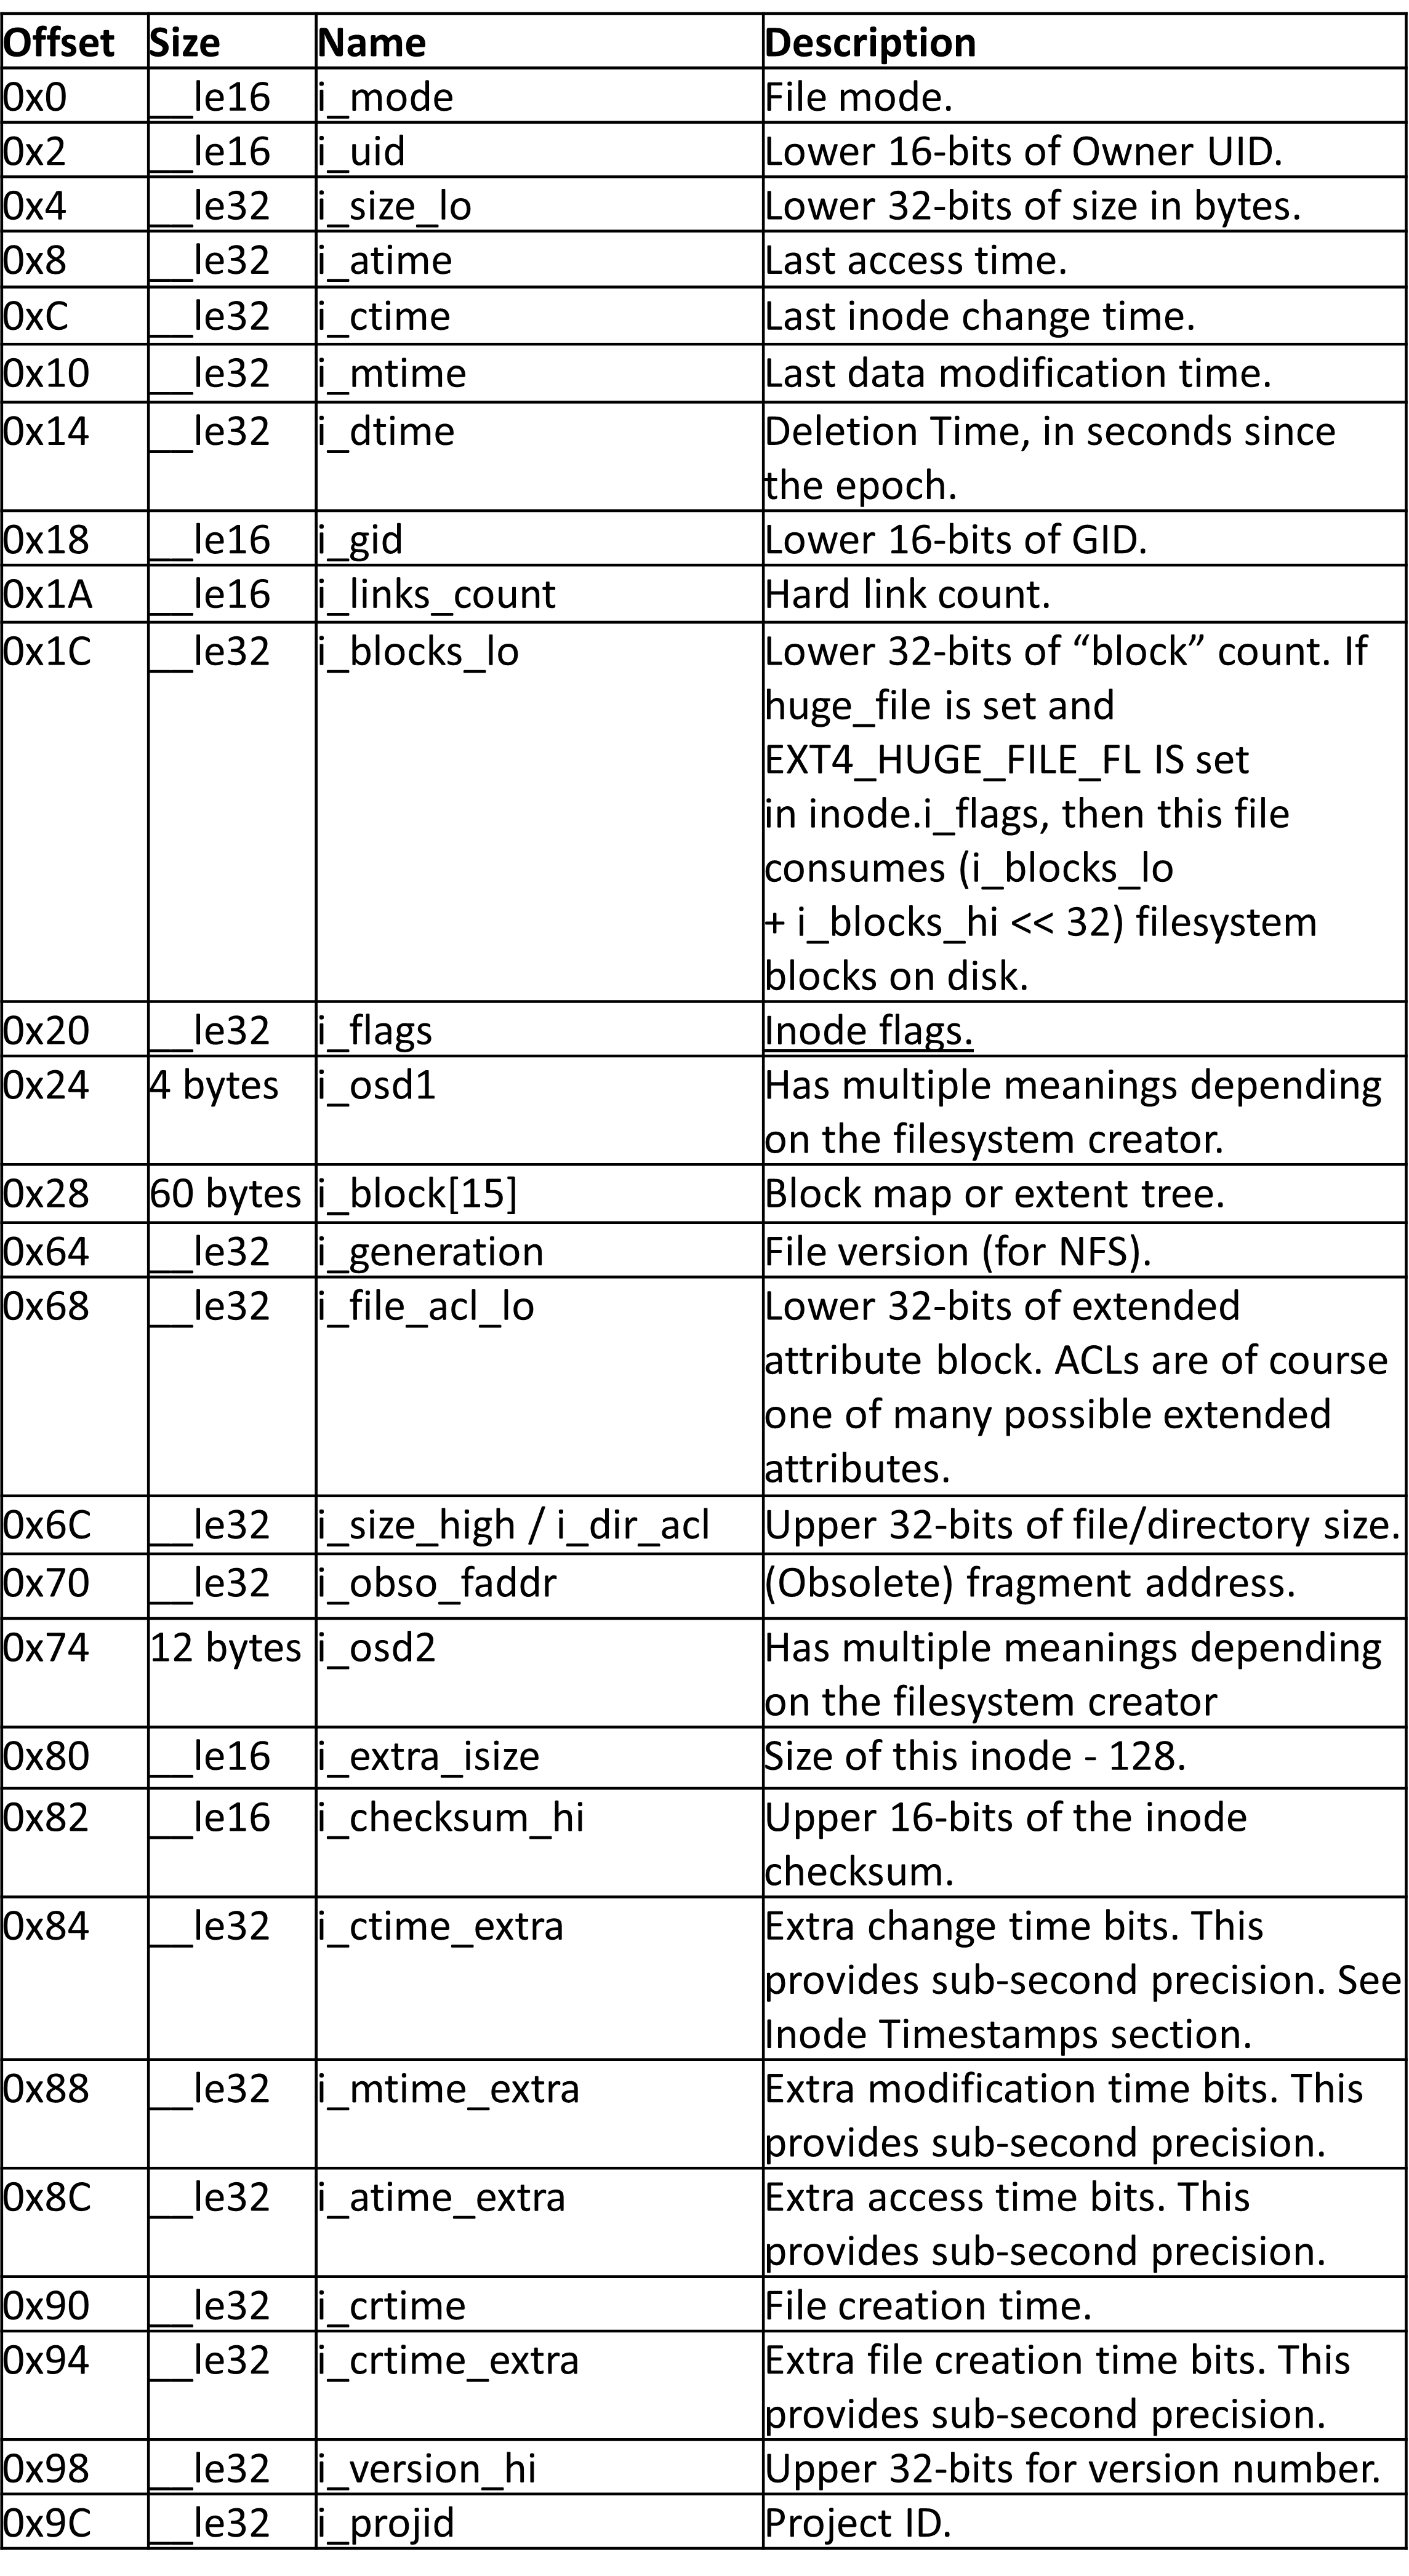
\includegraphics[width=\textwidth]{inode}
\end{center}

Lorsque vous utilisez des extensions, le tableau i\_block ne contient que les extensions elles-mêmes, alors qu'avec les blocs indirects, le tableau i\_block contient des pointeurs vers des blocs indirects, qui à leur tour contiennent des pointeurs vers des blocs de données. L'en-tête d'inode est également légèrement différent lors de l'utilisation d'étendues, car le champ i\_flags aura le bit EXT4\_EXTENTS\_FL défini.

\begin{center}
	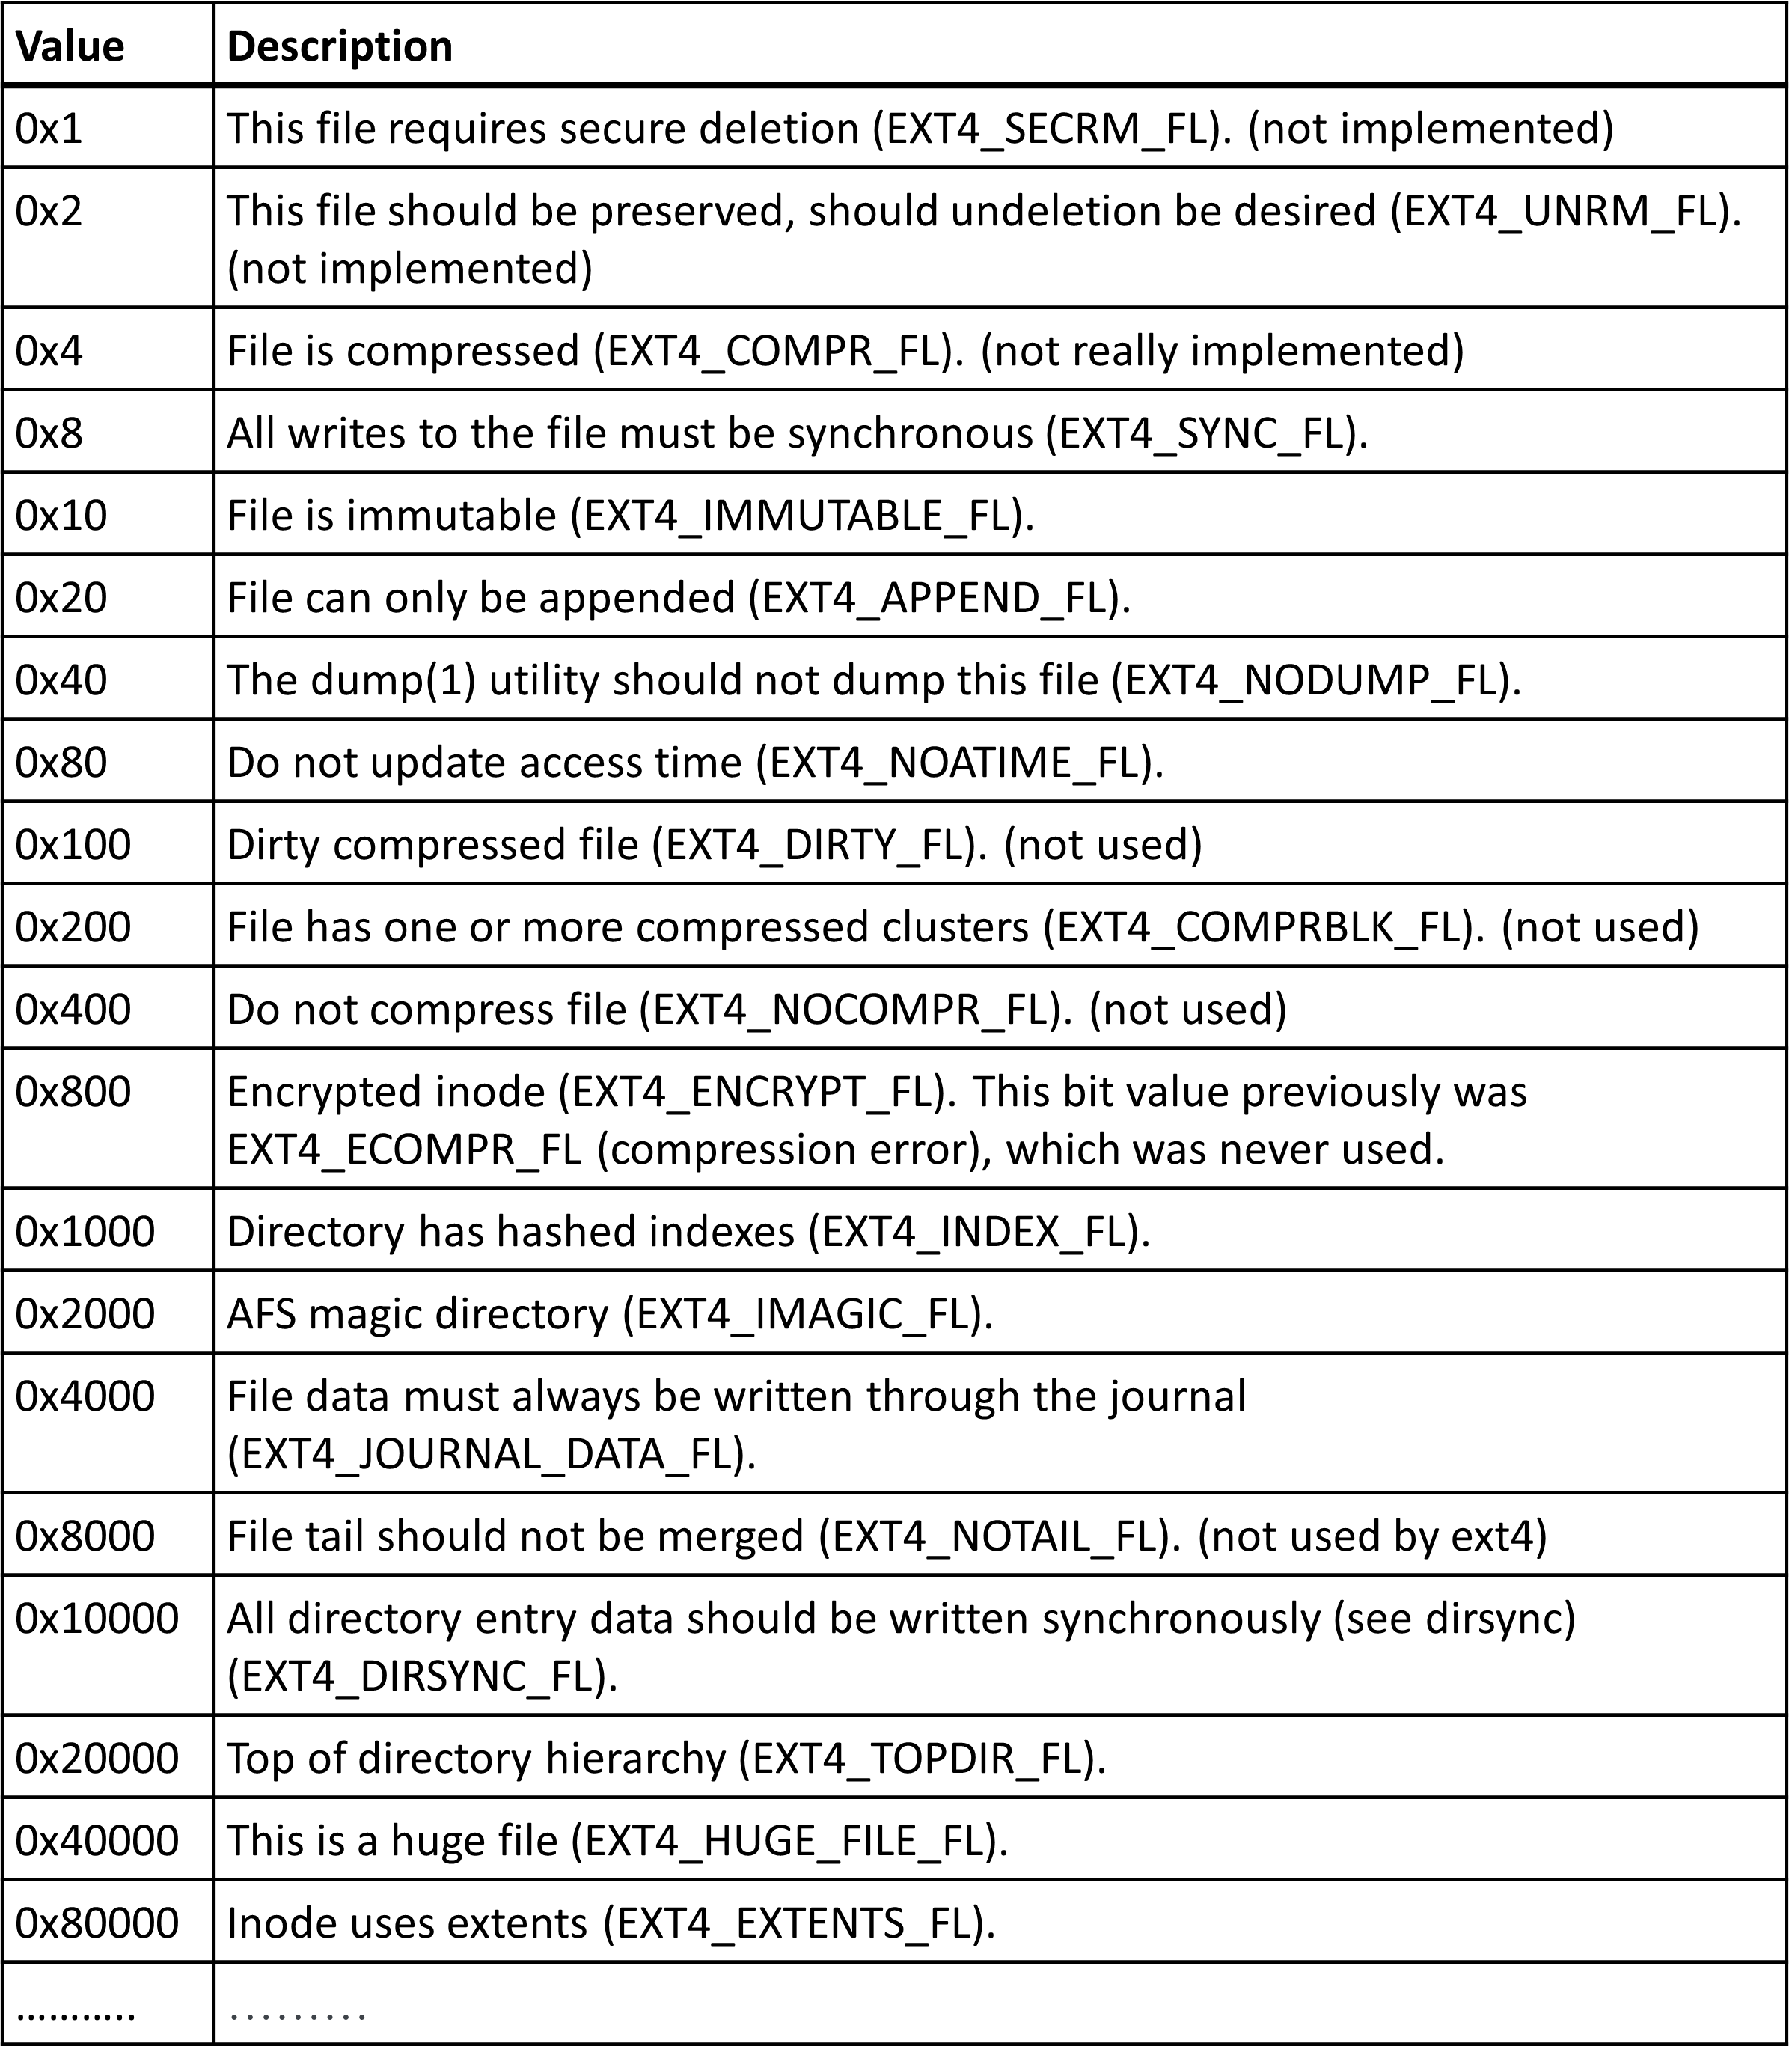
\includegraphics[width=\textwidth]{inode_flags}
\end{center}
\chapter{Les fonctionnalités d'ext4}
Ext4 est connu pour ses excellentes performances et son évolutivité, ce qui en fait un choix populaire pour de nombreux cas d'utilisation. Voici quelques fonctionnalités clés liées aux performances d'Ext4 :\newline
Les extents : Ext4 utilise un système de stockage de fichiers basé sur l'étendue, qui est plus efficace que le stockage traditionnel basé sur les blocs utilisé par les anciens systèmes de fichiers comme Ext2 et Ext3. Les étendues permettent des blocs de fichiers plus grands et plus efficaces, ce qui peut améliorer les performances de lecture et d'écriture.\newline
Allocation différée : Ext4 utilise l'allocation différée pour optimiser l'utilisation de l'espace disque. Au lieu d'allouer des blocs immédiatement lorsqu'un fichier est écrit, Ext4 retarde l'allocation jusqu'à ce qu'elle soit nécessaire. Cela permet à Ext4 d'allouer des blocs contigus, ce qui améliore les performances et réduit la fragmentation.\newline
Allocation multibloc : Ext4 propose une allocation multibloc, qui permet au système de fichiers d'allouer plusieurs blocs contigus à la fois. Cela peut améliorer considérablement les performances en réduisant le nombre de recherches de disque nécessaires pour lire et écrire des données.\newline
Journalisation : Ext4 propose la journalisation, qui fournit une couche supplémentaire de protection des données en enregistrant les modifications du système de fichiers avant qu'elles ne soient enregistrées sur le disque. Cela peut améliorer les performances en réduisant le besoin de vérifications de cohérence intensives sur le disque après une panne du système.
\section{Extents}
Les étendues (\textit{extents}) sont l'une des caractéristiques les plus importantes du système de fichiers \textit{ext4}. Dans \textit{ext3}, les données de fichier sont stockées dans une liste chaînée de blocs, alors que dans \textit{ext4}, les données de fichier sont stockées dans des étendues, permettant de réduire l'utilisation des blocs de métadonnées et d'améliorer l'efficacité du disque.

Sous l'ancien schéma, l'attribution d'une série contiguë de 1 000 blocs nécessite un bloc indirect pour mapper les 1 000 entrées ; avec les extensions, le mappage est réduit à une seule structure ext4\_extent avec ee\_len = 1000. Les étendues sont disposées sous forme d'arborescence. Chaque nœud de l'arbre commence par une structure ext4\_extent\_header. Si le nœud est un nœud intérieur, l'en-tête est suivi d'instances eh.eh\_entries de la structure ext4\_extent\_idx; chacune de ces entrées d'index pointe vers un bloc contenant plus de nœuds dans l'arborescence d'étendue. Si le nœud est un nœud feuille eh.eh\_depth == 0, alors l'en-tête est suivi d'instances eh.eh\_entries de la structure ext4\_extent; ces instances pointent vers les blocs de données du fichier. Le nœud racine de l'arborescence des étendues est stocké dans inode.i\_block, ce qui permet d'enregistrer les quatre premières étendues sans utiliser de blocs de métadonnées supplémentaires.

Le programme C suivant illustre l'utilisation des extensions dans ext4 :
\begin{center}
	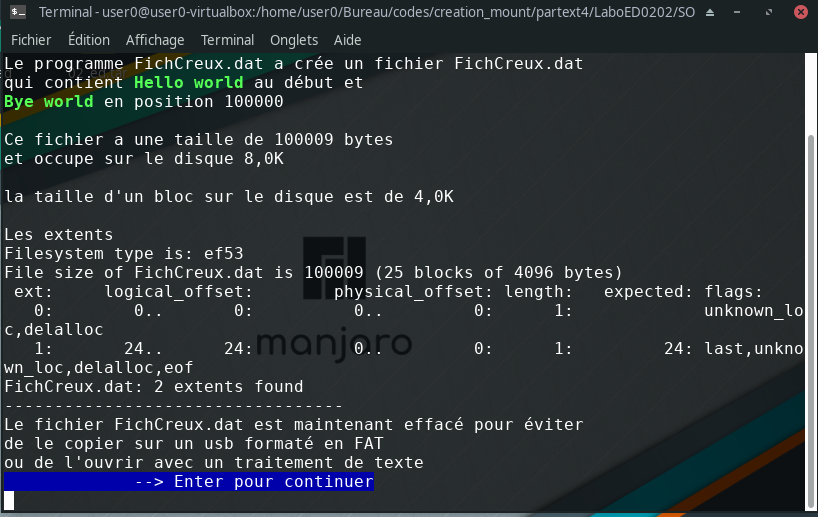
\includegraphics[width=\textwidth]{creux}
\end{center}

2 extents ont été utilisé pour créer le fichier FichCreux.dat.

\begin{center}
	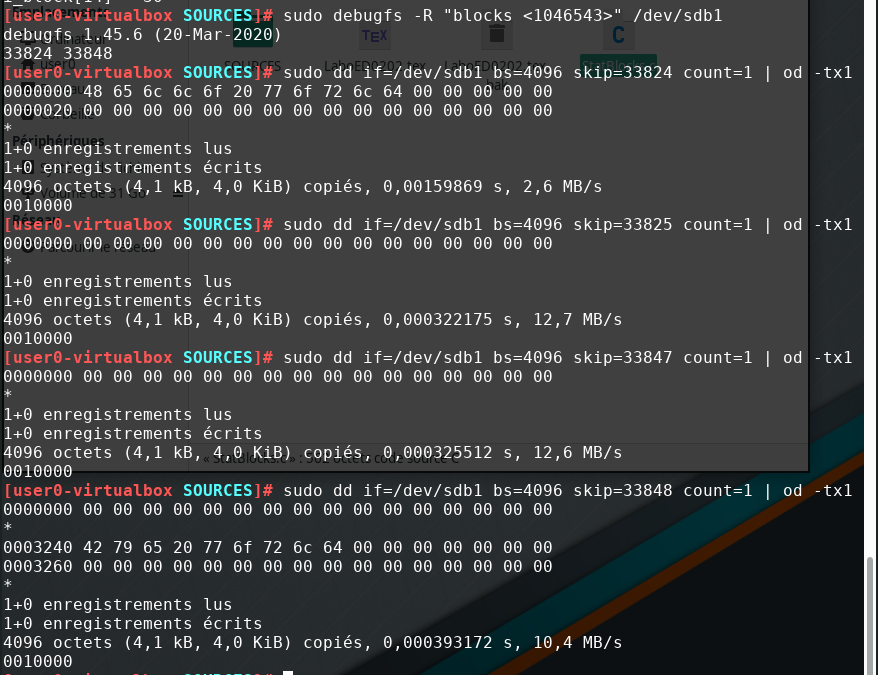
\includegraphics[width=\textwidth]{blockread}
\end{center}

Avec ls -i on a observé que l’inode du fichier est: 1046543.
debugfs -R “blocks <1046543>” /dev/sdb1 nous montre les adresses des blocks utilisés pour accueillir le contenu du fichier. On peut voir que les blocks sont contigus.
La commande dd nous permet de voir ce qui se trouve dans ces blocks. On peut voir que dans le premier block il y a le texte “Hello world” et dans le dernier il y a “Bye world”. Entre ces deux blocks se trouvent des blocks vides, non alloués.

\end{document}